\chapter{Functional aspects}
\label{sect:functional-aspects}

`And then you do that \ldots \emph{thing} \ldots in the air\ldots' I still remember one of the first rehearsals of \emph{Laserdance}, a dance piece with interactive sound that I was part of setting up. In the piece, the dancers could control the sound by moving in the air. None of us had a vocabulary to describe such sound-producing actions and resorted to talking about the `thing in the air.' I realized that we had to work on our terminology. In the following years, I spent quite some time reading up on the literature and trying to come up with a coherent taxonomy for describing the \emph{functional} aspects of various types of music-related body motion \citep{jensenius_musical_2010}. The taxonomy builds on the work by \citet{gibet_codage_1987}, combined with the proposals by \citet{cadoz_instrumental_1988}, \citet{delalande_gestique_1988}, and \citet{wanderley_gestural_2004}.
When I first developed my taxonomy, I used the term gesture extensively. After working more on the \emph{descriptive} terminology presented in the previous chapter, I have decided to use gesture more sparingly. There are times when it makes sense to talk about musical gestures, that is, actions with some intended/perceived meaning-bearing component. However, in many cases, it may be better to speak of motion or action.


\section{Four main types}

We can separate between four main functional categories of music-related body motion:

\begin{itemize}
\item \emph{Sound-producing} actions are the ones that produce sound. They can be subdivided into \emph{selection}, \emph{excitation}, and \emph{modification} actions.

\item \emph{Sound-facilitating} motion or actions are indirectly involved in the sound-production. They can be subdivided into \emph{support}, \emph{phrasing}, and \emph{entrainment} actions.

\item \emph{Sound-accompanying} motion or actions are not involved in sound production but follow one or more sound qualities. This includes \emph{sound-tracing}, \emph{sound-mimicking}, and \emph{air performance} actions.

\item \emph{Communicative} gestures are primarily extra-musical. These may be \emph{endogenous}, \emph{performer--performer} and \emph{performer--perceiver} types of communication, ranging from being communicative in a linguistic sense (\emph{emblems}), to being examples of more abstract forms of communication (\emph{expressive}).
\end{itemize}

These categories are not mutually exclusive. In most cases, they overlap in various ways. It may help to think of them as placed along an axis, as sketched in Figure~\ref{fig:action-link-sound}. This axis is inspired by the Kendon continuum \citep{mcneill_hand_1992} and shows that sound-producing actions are, by necessity, closely linked to the sound. The other types are more loosely (if at all) connected to the sound. In the following, we will look more at each of the four main types.

\begin{figure}[tbp]
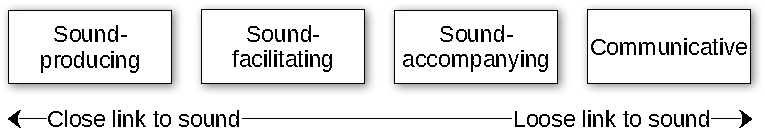
\includegraphics[width=\columnwidth]{figures/25-sound-link-crop.pdf}
\caption{A sketch of the relationship between the four different music-related body motion types and their connection to sound.}
\label{fig:action-link-sound}
\end{figure}


\section{Sound-producing actions}\label{sec:sound-producing-actions}

The first part of performing a sound-producing action on an instrument usually involves making a \emph{selection} of which key to press, which string to hit, and so on. This happens continuously during a performance on many instruments. There are also examples of selection actions performed before performing, such as changing the stops on an organ. Instruments constructed with many mechanical parts often afford more selection actions. One could argue that much of the preparation done in electro-acoustic instruments---such as selecting which presets to use or loading samples---could be seen as selection actions.

The actual sound-production is happening with an \emph{excitation} of the sound-producing element. In its purest form, an excitation action may be either \emph{direct} or \emph{indirect}. A direct excitation action is when the performer touches the sound-producing element with the body, such as blowing on a reed, plucking a string, or hitting a drum with the hand. Indirect excitation actions occur when an object is between the body and the sound-producing element, such as when playing with a bow, pick, or key.

\citet{godoy_reflections_2008} suggests that an excitation action can be decomposed into the main \emph{attack} preceded by a \emph{prefix} and followed by a \emph{suffix} (Figure \ref{fig:prefix-suffix}). The attack defines the sound and is largely based on the shape and quality of the prefix. The suffix is a continuation of the attack and typically works best if the performer can obtain fluidity through the whole action from the beginning of the prefix to the end of the suffix. In many cases, the suffix is also the preparation for the next attack. If played rapidly, the suffix of one action may overlap with the prefix of the next action according to coarticulation principles.

\begin{figure}[tbp]
	\centerline{
    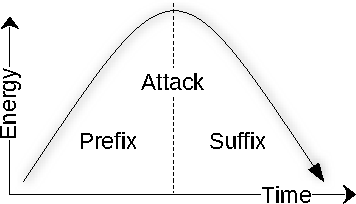
\includegraphics[width=0.5\columnwidth]{figures/26-prefix-suffix-crop.pdf}
    \caption{The excitation part of a sound-producing action may be seen as having an attack surrounded by a prefix and suffix \citep{godoy_reflections_2008}.}
		\label{fig:prefix-suffix}}
\end{figure}

The prefix, attack, and suffix are essential parts of a sound-producing action and are important for the perceiver. The prefix may guide the attention and set expectations for the sound to follow. For example, if a percussionist lifts a mallet high above a timpani, one would expect a loud sound. It is also expected that the rebound of the mallet (the suffix) matches the energy level of the prefix. As such, both prefixes and suffixes may help to `adjust' the perception of the sound based on ecological knowledge of the involved objects and actions.

When it comes to describing the quality of the sound-producing action, \citet{godoy_gestural-sonorous_2006} proposes three action--sound types based on the `sound object' classification by \citet{schaeffer_solfege_1967}:

\begin{itemize}
      \item \emph{Impulsive}: the excitation is based on a \emph{discontinuous} energy transfer, resulting in a rapid sonic attack with a decaying resonance. This is typical in percussion, keyboard, and plucked instruments.
      \item \emph{Sustained}: the excitation is based on a \emph{continuous} energy transfer, resulting in a continuously changing sound. This is typical for wind and (bowed) string instruments.
      \item \emph{Iterative}: the excitation is based on rapid and discontinuous energy transfers, resulting in sounds with successive attacks that are so rapid that they tend to fuse into perceptual chunks. This is typical in some percussion instruments, such as guiro and cabasa. It can also be found when one performs rapid attacks on other instruments, such as using the plectrum rapidly on a guitar.
\end{itemize}

As shown in Figure~\ref{fig:action--sound-time},  the action–sound types may be identified from the action and sound energy profiles. Sound is produced during the attack phase of the sound-producing action. Thus the prefix and suffix parts of the action are usually soundless, although there may be resonance in the instrument and reverb in the room.

\begin{figure}[tbp]
      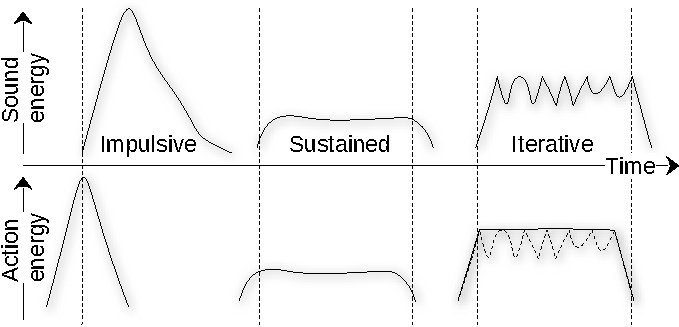
\includegraphics[width=1\textwidth]{figures/27-impulsive-sustained-crop.pdf}
\caption{Sketch of energy levels for actions and sound objects for the different types of sound-producing actions. The dotted lines indicate the attack phase. Iterative sound objects may result from a series of impulsive actions of the performer or a sustained action by the performer on an instrument that produces a series of impulsive actions.}
\label{fig:action--sound-time}
\end{figure}

Two action possibilities are sketched for iterative sounds in Figure~\ref{fig:action--sound-time}. Iterative sounds may result from either the instrument's construction or the action with which it is played. Percussion chimes can produce iterative sounds from continuous actions. Here the performer moves the hand with a sustained action over the rods, and it is the interaction of the moving rods that creates the iterative sound. Playing a tremolo on a piano, on the other hand, involves a series of iterative actions by the performer. Here, rapid actions fuse into one superordinate action based on coarticulation principles. In either case, iterative sounds and actions may be seen as having different properties than that of impulsive and sustained action--sound types.

The tripartite model sketched above is, of course, an over-simplification of a complex reality. For example, a violin may be played with many different excitation actions, and as documented by \citet{applebaum_art_1986} these may sometimes even merge. Sustained violin tones can be played with \emph{detaché}, in which the bow does not leave the string. The different types of \emph{martelé} bowing styles are based on short attacks but without the bow leaving the string, several of which can be categorized as an iterative sound character. In addition comes various types of impulsive sound types, including the finger plucking in \emph{pizzicato} playing. All these different playing styles also lead to different timbral nuances.

The world of electro-acoustic music has opened for even more sonic experimentation, often focusing on creating new \emph{timbres} and \emph{textures}. In the following, I will use timbre to denote the sonic quality of a perceived individual sound object, which can be thought of as the sound's `color.' I will use texture to refer to the combined sonic quality of multiple sound objects. So we could say that an instrument has a timbre, while an ensemble has a texture. In electro-acoustic music, it is not always possible to separate the two, and timbre and texture may seem as overlapping terms. Many composers and producers deliberately create new sonic timbres/textures that break with our traditional understanding of impulsive, sustained, and iterative sounds. For example, \citet{smalley_spectromorphology_1997} argues \emph{granular} sound is a sound type between sustained and iterative sounds. Working with digital signal processing or synthesis techniques makes it possible to create unnatural sounds, including sounds based on `reversing' traditional impulsive envelopes. As sketched in Figure~\ref{fig:impulsive-sustained}, it may then make more sense to think of a sound's energy profile as a continuum from more impulsive-like to more sustained-like sounds.

\begin{figure}[tbp]
	\centering
      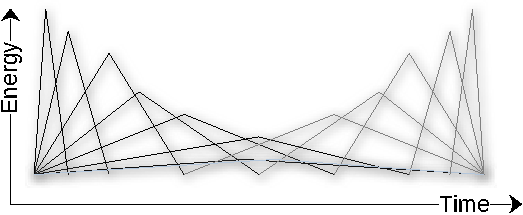
\includegraphics[width=0.7\textwidth]{figures/28-energy-time-crop.pdf}
\caption{A sketch of different types of attack--decay envelopes that can be found in electro-acoustic instruments, ranging from purely impulsive to purely sustained sounds, and including `reversed' sounds.}
\label{fig:impulsive-sustained}
\end{figure}

When it comes to the perception of sound objects, recent research by some of my colleagues at the University of Oslo shows that this is more complex than previously acknowledged. \citet{danielsen_where_2019} showed that the perceptual experience of an impulsive attack---the \emph{perceptual center} (P-center)---is not always easy to determine. Through perceptual experiments, they found that the P-center is usually somewhere before the energy peak. However, this depends on the timbral content and the temporal development of the sound object. Creating a machine listening system to detect such P-centers needs to include an understanding of the relationships between the differences between the physical sound, its signal-based representation, and the perception of where the attack is located \citep{lartillot_computational_2021}. This is challenging enough for impulsive sound objects and more so for sustained and iterative sounds with long and undulating development.

The third type of sound-producing action is that of \emph{modification} actions. As the name implies, these actions change the quality of the sound in one way or another. \citet{cadoz_instrumental_1988} suggests dividing such modification actions into two groups:

\begin{itemize}
\item \emph{Parametric}: actions that continuously change a parameter, such as a bow pressure in violin playing.
\item \emph{Structural}: actions that modify or change the object's structure, such as opening or closing a key on a wind instrument.
\end{itemize}

Many musical instruments are played with both excitation and modification actions, and in many instruments, the two types are easily separable. An example is string instruments in which the two hands play entirely different roles: the left hand mainly modifies the sound (choosing the pitch) while the right hand is carrying out the excitation. In wind instruments, the excitation is done in the mouth, and modification actions are carried out with the fingers.  There are also cases in which it is difficult to separate excitation and modification actions. \citet{kvifte_instruments_1989} argues that there are couplings between these two action types in wind instruments. The mouth can both produce sound and modify its quality. Similarly, string players use the left hand for selecting strings and modifying the pitch through the placement of fingers. However, the left hand can also be used for sound production. For example, string players can produce sound by pressing hard on a string with the left hand.


\section{Sound-facilitating actions}

The second main category of music-related body motion, \emph{sound-facilitating}, is not directly involved in sound production. Still, such motion or actions play an essential part in the shaping of the resultant sound. One sub-category here is \emph{support} actions. For example, hitting a piano key involves the hand, arm, and upper body. This multi-joint system is necessary to put the finger in motion, such that it hits the right key with a specific velocity at a particular point in time. Support actions may even have audible components. For example, \citet{wanderley_improving_1999} showed that clarinetists' sound-facilitating actions in the upper body had an audible component due to the instrument's changing sound diffusion pattern.

Performers' \emph{phrasing} actions are other types of sound-facilitating actions that directly impact the musical result, although they are not directly involved in the sound production. \citet{wanderley_evaluation_2002} showed that the sound-facilitating actions---what they called `ancillary gestures'---of clarinetists are an integral part of the instrumentalists' performance. Such sound-facilitating actions are remarkably stable and reproducible over time, probably because they are internalized as part of learning a piece  \citep{campbell_observation_2005}.

The third type of sound-facilitating actions is related to \emph{entrainment}, the synchronization of two or more independent rhythmic processes \citep{clayton_time_2005,clayton_interpersonal_2020}. Entrainment is typically seen in rhythmic music, in which a part of the body---for example, the foot---may synchronize with the music's pulse. Although bodily entrainment varies considerably between performers and performance styles, they may be thought of as necessary for the performance timing (or lack thereof). As such, entrained motion can be a generator of rhythm and timing, in the same way as the rhythm and timing in music can be a generator of motion \citep{clarke_body_1998}.

It is not always easy to differentiate between sound-producing and sound-facilitating actions. Although most musicians would probably not think about the difference between the two in performance, they would acknowledge the difference during rehearsal. I still remember how my first piano teacher asked me to put my hand on her wrist to feel how she moved her hand in a circular motion when playing arpeggios. The sound-facilitating actions are typically more visible than the sound-producing actions and are therefore also crucial for perceivers. Seeing a pianist playing with the elbows out to the sides, for example, is a different experience from holding the arms down along the sides. Furthermore, large phrasing actions in the upper body can be experienced as expressive gestures.


\section{Sound-accompanying actions}\label{sec:accompanying}

The third main category of sound-producing actions, sound-accompanying, is primarily focused on `following' qualities in the sound. More than 1500 years ago, \citet[p.8]{boethius_fundamentals_1989} wrote:

\begin{quote}
How does it come that when someone voluntarily listens to a song with ears and mind [\ldots] his body responds with motions somehow similar to the song heard?
\end{quote}

This question is equally valid today, and it has received renewed interest in recent music cognition studies. At the University of Oslo, we have contributed with several studies on \emph{sound-tracing}. This is a type of sound-accompanying motion based on representing perceived sound features in the air with the hand. When hearing a tone with a rising pitch, many people will spontaneously move a hand upwards. Coincidentally, many people would also say that the pitch `goes up,' an example of a bodily metaphor related to a sonic feature. To understand more about such relationships between people's spontaneous body motion and musical sound, we carried out a study in which we asked participants to `draw' the sound they heard on a graphic tablet \citep{godoy_exploring_2006}. The aim was to see what sound features the participants would respond to and trace with a digital pen. It turned out that people used several different strategies, which could be summarized as either:

\begin{itemize}
      \item mimicking the sound-producing action(s), such as quickly pressing down for impulsive sounds and `bowing' for sustained sounds.
      \item drawing one or more sound features, such as the dynamic envelope or the pitch contour.
      \item drawing an abstract shape, with some metaphoric content, such as `lifted' or `floating.'
\end{itemize}

Some of these alternatives are related to specific features present in the sound itself. Others focus on imagery of the sound-producing action. Others again were entirely metaphorical. In addition to tracing individual sounds, participants were also exposed to composite sounds consisting of multiple attacks or partly overlapping spectral features. One example of some responses to such a task can be seen in Figure~\ref{fig:sound-tracing}. Here we found, unsurprisingly, that more musically trained participants identified and traced the different parts of the composite sounds better than untrained participants.

\begin{figure}[tbp]
      \centering
      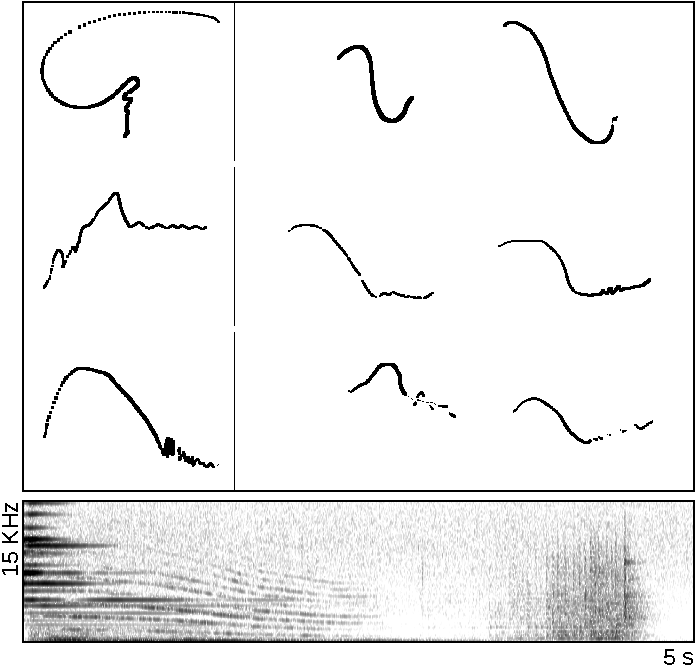
\includegraphics[width=\columnwidth]{figures/29-sound-tracing-crop.pdf}
      \caption{Nine tracings to a complex sound, composed of a long, downwards moving slide, followed by a short, rattle sound at the end. Musically trained participants typically traced both of the sonic objects, while less musically trained participants followed only the main envelope of the sound \citep{godoy_exploring_2006}.}
      \label{fig:sound-tracing}
\end{figure}

Moving the sound-tracing paradigm into three-dimensional space, \citet{nymoen_methods_2013} conducted sound-tracing experiments where the participants would move two hands in the air to short, synthetic sound objects. The motion capture analyses revealed a high correlation between the pitch height of the sound and the hands' vertical position. \citet{kelkar_computational_2019} continued this line of research but with musical material. She carried out a series of sound-tracing studies using speechless, sung melodies from four musical genres: classical vocalize, jazz scat, Sámi folk music, and a North Indian rag. She found that some participants related pitch height to vertical hand position. However, the main finding was that several other motion strategies were also used, summarized in Figure~\ref{fig:sound-tracings-kelkar}.

\begin{figure}[tbp]
      \centering
      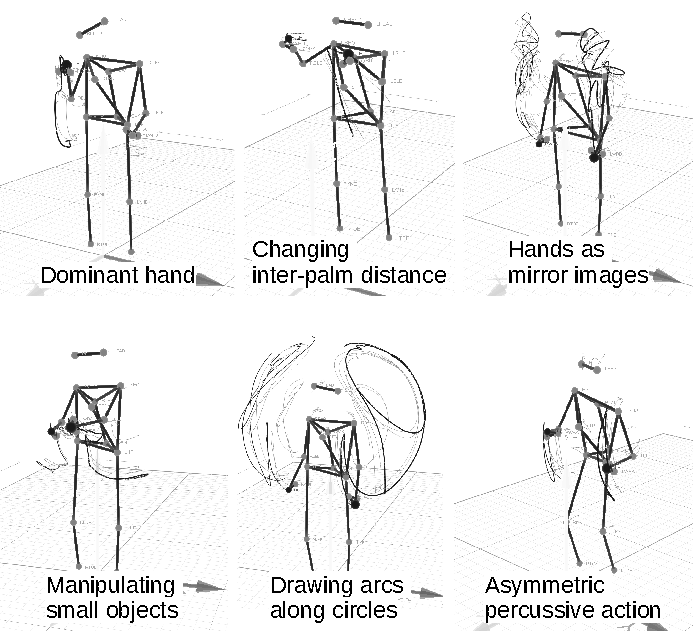
\includegraphics[width=\columnwidth]{figures/30-sound-tracing2-crop.pdf}
      \caption{Motion history images exemplifying the six dominant sound-tracing strategies in a study by \citet{kelkar_analyzing_2018}.}
      \label{fig:sound-tracings-kelkar}
\end{figure}

While most of our sound-tracing studies have focused on individual sound objects or melodies, we have also experimented with sound-accompanying actions to rhythmic music. In a study of people's ability to synchronize a 'virtual shaker' to music, participants were asked to move a short wooden stick in the air \citep{danielsen_moving_2015}. As expected, most participants were able to do this effortlessly when the rhythm was clear and easy to follow. However, moving to stimuli with micro-rhythmic variations was challenging for most participants. Only some musically trained participants managed to achieve a high level of synchronization with these patterns.

Another type of sound-accompanying action we have studied is that of `air performance.' While the sound-tracing paradigm primarily investigates peoples' ability to follow sound features, air performance mimics imagined sound-producing actions. In an `air piano' experiment, participants were asked to spontaneously play piano in the air, as if producing the music they heard \citep{godoy_playing_2006}. The analyses revealed that participants were able to perform the task regardless of musical training. The main difference was that musically trained participants showed a higher level of detail to onsets and register than the novices. The latter primarily followed the music's general contour. Perhaps the most exciting finding was that even people that claimed to be `tone-deaf' and `unmusical' managed to complete the task relatively well.

\emph{Dancing} is another example of sound-accompanying motion, and asking people to dance freely to music can tell about how they experience the music.
In a series of free-dance studies, we looked at how individual dancers follow musical patterns \citep{jensenius_actionsound_2007,haga_correspondences_2008}. Since we asked the dancers to repeat their improvisations to the same musical material three times, we also studied similarities and differences between each participant's performance. These studies found a correlation between pitch height and vertical motion, albeit weaker than in the sound-tracing experiments. More importantly, we found correlations between physical effort and the spectral complexity and loudness of the sound.

Dancing usually happens in a social setting. To understand more about the inter-subjectivity of dance experiences, we set out to study how groups of people dance together in a club-like environment \citep{solberg_pleasurable_2017,solberg_group_2019}. One aim was to understand more about the social dynamics of the groups, which consisted of up to ten people at a time. We were also interested in looking at the effect of the `break routine' typically found in electronic dance music (EDM). This is a moment in which the regular pulse dissolves, followed by a gradual pitch rise accompanied by an increase in the timbral/textural complexity of the mix. The break routine ends when the beat is `dropped' back, and the groove continues. We found that the break routine did, indeed, influence the dancers' rhythmic motion patterns. We also found that the reintroduction of the groove after the drop `re-energized' the group.

In parallel to studying large-scale sound-accompanying motion and action, I have run studies on music-related \emph{micromotion} \citep{jensenius_exploring_2017,gonzalez_sanchez_correspondences_2018,gonzalez_sanchez_analysis_2019,zelechowska_headphones_2020}. Using a `standstill' paradigm, the participants have been asked to stand as still as possible on the floor for 6--10 minutes while listening to (musical) sound and silence in randomized order. Of course, it is impossible to stand completely still, and we have been measuring people's micromotion level using an optical motion capture system. By playing different types of music to people when they stand still, we can learn more about the different motion-inducing effects of the music in question. Not surprisingly, we have found that dance music with a regular beat pattern most significantly influences the micromotion. However, how and why this is the case are still open questions.


\section{Communicative gestures}

The fourth main category of music-related body motion is that of \emph{communicative} gestures. I call these gestures since they are focused on communicating meaning in one way or another. Communicative gestures may be endogenous, but they are often used to communicate between performers or between performers and perceivers. Such gestures can be communicative in a linguistic sense (emblems) or abstract (expressive). The way a performer communicates with an audience is often critical for how the concert is experienced. Equally important is performer--performer communication, which may involve anything from glancing at each other to support the continuous adjustments of musical features throughout the flow of performance to actions that resemble conductor messages \citep{timmers_together_2022}. With the advancement of new tracking technologies, it is now possible to empirically study performer--performer communication. For example, eye-tracking studies of a string quartet reveal how the other musicians look at the first violinist throughout a performance \citep{bishop_move_2021}.

The \emph{conductor} is a musicking actor that has received little attention in this book so far. It may perhaps be more relevant to talk about the \emph{musical leader} to also include people without the institutionalized title `conductor.' Such a musical leader can be the first violinist of a string quartet, the founder of a jazz band, the lead singer in a pop/rock band, or the conductor of a full-size orchestra. The focus on gestural communication is what differentiates the musical leader from the other members of an ensemble.  \citet[p.243]{davidson_body_2002} describe how Annie Lennox leads her band:

\begin{quote}
She is a narrator-interpreter in her use of illustrative and emblematic gestures with the co-performers and audience. She is a co-worker in her use of regulatory movements to coordinate musical entrances and exits.
\end{quote}

\citet{leante_gesture_2014} argues that khyal singers in North Indian classical music communicate the lyrics through iconics or metaphorics, and perform abstract gestures along with the flow of the improvised sections. However, musical leadership is not always connected to a particular person. \citet{mccaleb_embodied_2014} describes how the leadership varies within a string quartet, what he refers to as the `fluidity of ensemble roles.' While such musical leadership is possible in relatively small ensembles, larger ensembles often rely on a traditional conductor engaging in what \citet{volpe_measuring_2016} call ‘sensorimotor conversations’ with the musicians. A conductor can be seen as a communicator of emotional content, besides providing temporal and structural information to the musicians. We will return to the conductor's role in a discussion about the orchestra as `instrument' in Chapter~\ref{sec:orchestra}.

I find it intriguing that new motion tracking technologies make it possible to perform `in the air.' Then it is possible to use communicative gestures for sound production and modification. However, what are meaningful mappings between motion and sound? How does one extract actions from the continuous motion signal? How does one interpret the meaning of gestures from the segmented actions? How does such a shift in function from communication to sound-production challenge expectations about how sound is produced and modified? We will return to such questions when discussing air instruments in Chapter~\ref{chap:touchless}.
